\documentclass[conference]{IEEEtran}
\IEEEoverridecommandlockouts

\usepackage{cite}
\usepackage{amsmath,amssymb,amsfonts}
\usepackage{graphicx}
\usepackage{textcomp}
\usepackage{xcolor}

% make sure captions are small font
\usepackage{subcaption}
\usepackage{caption}
\captionsetup{font=small}
\captionsetup[sub]{font=small}

\def\BibTeX{{\rm B\kern-.05em{\sc i\kern-.025em b}\kern-.08em
    T\kern-.1667em\lower.7ex\hbox{E}\kern-.125emX}}

\begin{document}

\title{Mixed-Integer Convex Programming for \\Motion Planning in Dual-Arm Manipulation}

\author{\IEEEauthorblockN{Phone Thiha Kyaw and Karyna Volokhatiuk}
\IEEEauthorblockA{\textit{University of Toronto Institute for Aerospace Studies} \\
Email: \{phone.thiha, karyna.volokhatiuk\}@robotics.utias.utoronto.ca}
}

\maketitle

\begin{abstract}
Motion planning for high-degree-of-freedom robotic manipulators is challenging due to complex constraints such as collision avoidance, kinematic limits, and trajectory smoothness.
%
In this project, we propose formulating the motion planning problem for dual-arm manipulation (14-DOF) as a convex optimization problem.
%
Specifically, we will leverage the recently studied Graph of Convex Sets (GCS) framework~\cite{marcucci2024shortest} to model motion planning as a compact mixed-integer optimization problem, similar to~\cite{marcucci2023motion}.
%
To evaluate its effectiveness, we will compare our approach against classical sampling-based motion planners from OMPL~\cite{sucan2012open}.
%
The proposed method will be implemented and tested in Drake~\cite{drake}, a widely used toolbox for modeling and simulating robotic systems.
\end{abstract}

\section{Background}

Motion planning is a fundamental problem in robotics that involves computing a feasible and efficient trajectory for a robot to move from an initial configuration to a goal configuration while satisfying various constraints\cite{lavalle2006planning}.
%
The problem becomes particularly challenging in high dimensional systems, which are generally known to be PSPACE-hard\cite{reif1979complexity}.

Classical approaches to motion planning rely heavily on sampling-based planners, such as Rapidly-exploring Random Trees (RRT)\cite{lavalle2001randomized} and Probabilistic Roadmaps (PRM)\cite{kavraki1996probabilistic}, due to their ability to efficiently explore high-dimensional spaces.
%
These planners have been widely adopted because they can handle complex environments without requiring an explicit representation of the free space.
%
However, when additional constraints such as kinodynamic feasibility, obstacle avoidance, or motion continuity are introduced, these methods struggle to produce high-quality, optimal trajectories.

Recent advances in optimization-based motion planning have tackled these limitations by formulating the problem as a compact mixed-integer convex program\cite{marcucci2023motion}.
%
One such approach, the Graph of Convex Sets (GCS) framework\cite{marcucci2024shortest}, enables the encoding of collision-avoidance constraints and system dynamics within a single convex optimization formulation.
%
By leveraging convex relaxations and mixed-integer programming, GCS provides a structured way to computing globally optimal trajectories while ensuring feasibility in constrained environments.

\begin{figure}[!t]
    \centering
    \begin{subfigure}[b]{0.23\textwidth}
        \centering
        \fbox{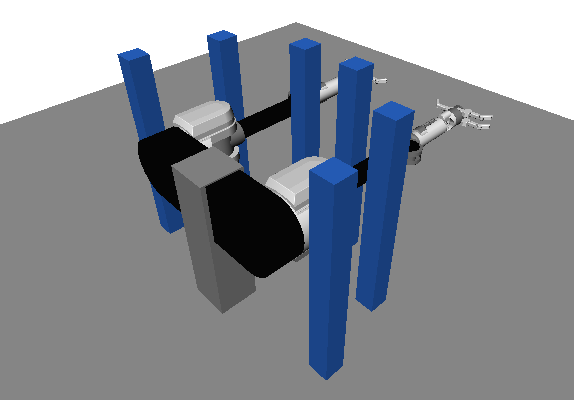
\includegraphics[width=\textwidth]{figures/cage_start_orbit.png}}
        \captionsetup{justification=centering}
        \caption{Start configuration}
        \label{subfig:cage_start_orbit}
    \end{subfigure}\hspace{0.01\textwidth}
    \begin{subfigure}[b]{0.23\textwidth}
        \centering
        \fbox{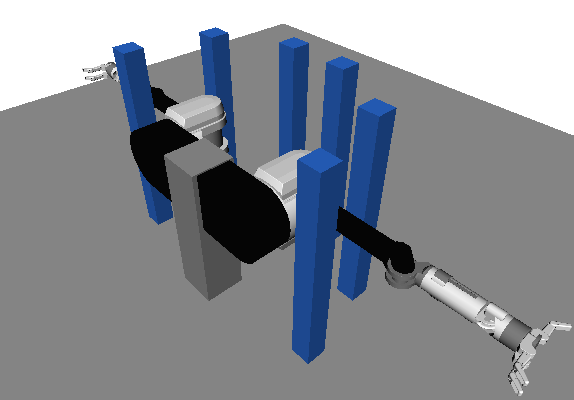
\includegraphics[width=\textwidth]{figures/cage_goal_orbit.png}}
        \captionsetup{justification=centering}
        \caption{Goal configuration}
        \label{subfig:cage_goal_orbit}
    \end{subfigure}
    \caption{A dual-arm manipulation problem for the Barrett WAM Arm in $\mathbb{R}^{14}$, simulated in Drake. Starting with both arms pointing in the same direction (a), they must be moved to extend outward in opposite directions without hitting the cage (b).}
    \label{fig:simulation}
\end{figure}

\section{Contributions}
In this project, we explore the use of the GCS framework for kinodynamic motion planning in dual-arm robotic manipulation.
%
Our key contributions include:
\begin{itemize}
    \item We formulate the problem of finding \textit{collision-free, kinodynamic motion plans} for a dual-arm manipulator as a mixed-integer convex program, similar to~\cite{marcucci2023motion}.
    %
    Unlike prior work, our study considers the scalability of the framework in significantly higher-dimensional systems---14 degrees of freedom in this case (Figure~\ref{fig:simulation}).
    %
    \item We extensively evaluate our optimization-based approach against classical sampling-based motion planners from the Open Motion Planning Library (OMPL)~\cite{sucan2012open}, analyzing key performance metrics such as computation time, solution quality, and success rate.
\end{itemize}

\bibliographystyle{IEEEtran}
\bibliography{IEEEabrv,main}

\end{document}
